\documentclass[11pt,a4paper]{article}
\usepackage[utf8]{inputenc}
\usepackage[T1]{fontenc}
\usepackage[a4paper,margin=1in]{geometry}
\usepackage{amsmath,amssymb}
\usepackage{booktabs}
\usepackage{tabularx}
\usepackage{array}
\usepackage{longtable}
\usepackage{graphicx}
\usepackage{float}
\usepackage{caption}
\usepackage{xcolor}
\usepackage{enumitem}
\usepackage{fancyhdr}
\usepackage{tikz}
\usetikzlibrary{shapes.geometric,arrows.meta,positioning,fit,backgrounds,calc}
\usepackage[hidelinks]{hyperref}

\definecolor{accent}{HTML}{1F4E79}
\definecolor{soft}{HTML}{F2F4F7}
\definecolor{rule}{HTML}{B9C2CC}
\definecolor{ok}{HTML}{2E7D32}
\definecolor{bad}{HTML}{B3261E}

\pagestyle{fancy}
\fancyhf{}
\renewcommand{\headrulewidth}{0.4pt}
\fancyhead[L]{\small\itshape ThinkStack}
\fancyhead[R]{\small\itshape \leftmark}
\fancyfoot[C]{\small\thepage}

\setlist{itemsep=2pt, topsep=4pt}

\newcommand{\coverpage}[2]{%
\begin{titlepage}
\centering
{\large CHRIST (Deemed to be University), Bengaluru\par}
{\large Department of Computer Science\par}
\vspace{1.1cm}
{\Large\bfseries #1\par}
\vspace{0.35cm}
{\large Course: CSC481-5, Computer Science Project\par}
{\large Semester V\par}
\vspace{1.5cm}
{\Huge\bfseries ThinkStack\par}
\vspace{0.35cm}
{\large\itshape #2\par}
\vspace{1.5cm}
{\large\bfseries Submitted by\par}
\vspace{0.3cm}
\begin{tabular}{clc}
\toprule
\textbf{Sl. No.} & \textbf{Student Name} & \textbf{Register No.} \\
\midrule
1. & Aditya Mehta & 2440204 \\
2. & Jitvan Chadha & 2440222 \\
3. & Ritesh K R & 2440233 \\
\bottomrule
\end{tabular}
\vspace{1.2cm}

\begin{tabular}{ll}
\textbf{Guide:} & Dr. New Begin \\
\textbf{Class:} & 5BSC CS \\
\textbf{Repository:} & \texttt{github.com/get-thinkstack/ThinkStack} \\
\end{tabular}
\vfill
{\large July 2026\par}
\end{titlepage}
}

\newcommand{\evidence}[1]{%
\begin{center}
\fcolorbox{rule}{soft}{\parbox{0.93\linewidth}{\small #1}}
\end{center}}

\newcommand{\yes}{\textcolor{ok}{\textbf{Yes}}}
\newcommand{\no}{\textcolor{bad}{\textbf{No}}}

\begin{document}
\coverpage{Sprint II: Design and Development Document}{Packaging, Distribution and Verified Delivery}

\tableofcontents
\newpage

\section{Sprint Overview}
\markboth{Sprint Overview}{}

\subsection{Period and scope}

Sprint II ran from 7 July 2026 to 30 July 2026. Sprint I produced an
application that worked on the machines it was written on. Sprint II addressed
a different problem: making that application installable and correct on a
machine the team has never seen.

\begin{center}
\small
\begin{tabular}{@{}ll@{}}
\toprule
\textbf{Attribute} & \textbf{Value} \\
\midrule
Duration & 7 July 2026 to 30 July 2026 \\
Active development days & 12 \\
Commits & 106 \\
Pull requests merged (project total) & 42 \\
Deliverable & signed, validated installers for three operating systems \\
\bottomrule
\end{tabular}
\end{center}

The team worked jointly, with interface work, backend correction, and release
engineering proceeding in parallel and integrating through pull requests.

\subsection{Sprint goal statement}

\evidence{\textbf{Goal.} A person who has never installed a developer tool
should be able to download one file, run it, and have every feature work,
including on a computer with no Python, no model runtime, and no LaTeX
distribution, and with the network disconnected.}

\section{Design Problem: The Unprepared Machine}

Sprint I made an implicit assumption that a developer machine and a user
machine are alike. They are not, and every significant defect of this sprint
came from that single assumption.

\begin{center}
\small
\begin{tabularx}{\linewidth}{@{}lXX@{}}
\toprule
\textbf{Resource} & \textbf{Developer machine} & \textbf{User machine} \\
\midrule
Python runtime & installed, correct version & absent \\
Model weights & present in the working directory & absent \\
Embedding weights & cached from earlier downloads & absent \\
TeX distribution & installed & absent \\
Working directory & the project checkout & arbitrary \\
Network & available & may be absent by design \\
\bottomrule
\end{tabularx}
\end{center}

The design response was to make the installer self-contained, and then to build
automation that proves it, because human inspection had already been shown to be
unreliable.

\section{Design of the Distribution System}

\subsection{Packaging architecture}

\begin{figure}[H]
\centering
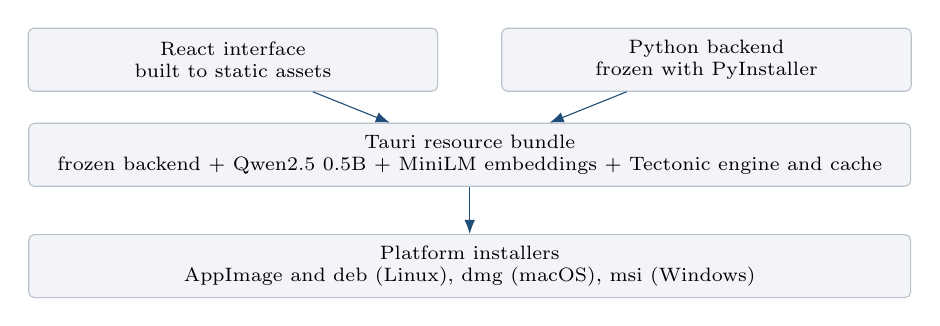
\begin{tikzpicture}[
  node distance=6mm,
  box/.style={draw=rule, fill=soft, rounded corners=2pt, minimum height=8mm,
              inner xsep=3mm, align=center, font=\scriptsize},
  arr/.style={-{Latex[length=1.8mm]}, draw=accent}
]
\node[box, minimum width=52mm] (fe) {React interface\\built to static assets};
\node[box, minimum width=52mm, right=8mm of fe] (py) {Python backend\\frozen with PyInstaller};
\node[box, minimum width=112mm, below=8mm of $(fe)!0.5!(py)$] (res) {Tauri resource bundle\\
  \scriptsize frozen backend + Qwen2.5 0.5B + MiniLM embeddings + Tectonic engine and cache};
\node[box, minimum width=112mm, below=of res] (inst) {Platform installers\\
  \scriptsize AppImage and deb (Linux), dmg (macOS), msi (Windows)};
\draw[arr] (fe) -- (res); \draw[arr] (py) -- (res); \draw[arr] (res) -- (inst);
\end{tikzpicture}
\caption{Packaging pipeline. Every runtime dependency is placed inside the resource bundle.}
\end{figure}

\paragraph{Directory packaging rather than single-file.} PyInstaller was
configured to emit a directory rather than a single executable. A single-file
build extracts its entire payload to a temporary directory on every launch,
which for a bundle approaching one gigabyte would impose that cost each time the
application starts.

\paragraph{Read-only and writable roots separated.} The bundle is read only once
installed, so the design distinguishes the shipped payload from the user's
state. Model weights and the TeX cache are copied from the bundle into the
user's data directory on first use.

\subsection{Release channel design}

\begin{center}
\small
\begin{tabular}{@{}llll@{}}
\toprule
\textbf{Channel} & \textbf{Branch} & \textbf{Tag form} & \textbf{Audience} \\
\midrule
stable & \texttt{main} & \texttt{vX.Y.Z} & the public \\
beta & \texttt{beta} & rolling tag \texttt{beta} & invited testers \\
nightly & any & rolling tag \texttt{nightly} & internal \\
\bottomrule
\end{tabular}
\end{center}

Branches never produce installers. Only a tag does. A release therefore cannot
occur accidentally through a merge, and the expensive three-platform build is
paid only when it is intended.

\subsection{Release guardrails}

Each guardrail exists because the corresponding mistake is not reversible once
an installer is published.

\begin{center}
\small
\begin{tabularx}{\linewidth}{@{}lX@{}}
\toprule
\textbf{Refusal condition} & \textbf{Reason} \\
\midrule
working tree not clean & uncommitted work would not be in the build \\
tag already exists & re-tagging changes the meaning of a version silently \\
version lower than published & the updater would move installed applications backwards \\
CI not green for that commit & a tag builds installers, so a red commit ships broken \\
any asset near 2 GiB & the hosting platform rejects it after a long build \\
\bottomrule
\end{tabularx}
\end{center}

\section{Implementation}

\subsection{Phase 1: packaging and delivery, 7 to 24 July}

\begin{itemize}[leftmargin=*]
  \item A public download page was produced and deployed.
  \item Cross-platform builds were automated for Linux, macOS and Windows from a
        single configuration file, so adding a platform is a data change rather
        than a workflow change.
  \item Hardware-aware model routing was introduced, selecting a model against
        currently available memory rather than installed memory, on the
        assumption that the user is running other software.
  \item In-application updates were implemented against signed release
        manifests, with per-channel endpoints so a beta installation updates
        within the beta channel.
  \item Linux packaging was moved to \texttt{appimagetool} after the default
        tool proved unable to resolve the libraries vendored inside the frozen
        Python bundle.
\end{itemize}

\subsection{Phase 2: quality infrastructure, 25 to 29 July}

\begin{itemize}[leftmargin=*]
  \item An automated test suite was introduced, growing to 309 tests across 23
        modules.
  \item Hardware diagnosis was reimplemented in Rust inside the desktop shell.
        The previous implementation imported a deep learning framework purely to
        probe for a GPU, adding several seconds to every launch.
  \item A local verification gate was written that mirrors the continuous
        integration configuration exactly, so a developer sees the same result
        locally that the server will produce.
  \item Git hooks were installed from a version-controlled directory, so the
        whole team runs identical checks and updates arrive with a normal pull.
  \item Model discovery across runtimes was added, so weights already present
        through other local tools are reused rather than downloaded again. This
        required a canonical naming key, because the same weights are named
        differently by each runtime.
\end{itemize}

\subsection{Phase 3: release, failure and correction, 29 to 30 July}

Three releases were published. The third, version 1.0.0, did not work.

\evidence{\textbf{Observed failure.} The published v1.0.0 installer displayed a
loading screen indefinitely. Continuous integration was green throughout,
because every test exercised the source tree and no test had ever launched the
packaged application.}

\section{Root Cause Analysis}

\subsection{Why the application did not start}

Three defects compounded, each concealing the next.

\begin{enumerate}[leftmargin=*]
  \item \textbf{The backend could not be located.} The packaging tool installs
        the executable into one directory and its resources into another. The
        lookup searched only beside the executable, so inside the installed
        application it found nothing and fell back to its development path:
        launching a system Python interpreter.
  \item \textbf{The fallback interpreter was already broken.} The Linux
        application image exports an environment variable that redirects a
        Python interpreter's standard library search into the mounted image. A
        frozen interpreter ignores this; a system interpreter does not. It
        terminated before executing any project code.
  \item \textbf{The failure was invisible.} The loading screen retried without
        limit and had no error state, so a backend that died in under a second
        was indistinguishable from one that was merely slow.
\end{enumerate}

\subsection{Further defects found in the same investigation}

\begin{itemize}[leftmargin=*]
  \item The embedding weights were never placed in the bundle, so the first
        document ingested on an installed copy attempted a network download.
  \item The model directory was derived from the current working directory,
        which the application image changes before launching. The path resolved
        to a location that did not exist while the model sat inside the bundle.
        This was incorrect on every operating system for every installed copy.
  \item The window terminated roughly one second after appearing on the test
        system, caused by heap corruption in a graphics path of the system
        webview.
  \item The paper writer required a TeX distribution that no ordinary machine
        has, and was routed to two fine-tuned models that are never built, so it
        silently used the weakest model available.
\end{itemize}

\subsection{Corrections applied}

\begin{center}
\small
\begin{tabularx}{\linewidth}{@{}lX@{}}
\toprule
\textbf{Defect} & \textbf{Correction} \\
\midrule
backend not found & resource location is obtained from the packaging framework, with explicit fallbacks per packaging format \\
interpreter poisoned & interpreter-controlling variables are removed from the child environment \\
failure invisible & startup is bounded, each step is reported with timings, and the trace is written to a log file that outlives the window \\
embedding weights absent & weights are staged into the bundle at build time \\
model path from cwd & the backend resolves its own paths; the shell no longer overrides them \\
window crash & the failing renderer path is disabled on the affected platform \\
TeX absent & a TeX engine and a warmed package cache are shipped in the installer \\
weak model for LaTeX & routing prefers the larger model when it is present and fits memory \\
\bottomrule
\end{tabularx}
\end{center}

\section{Design of the Verification System}

The corrective work was not limited to the defects. The failure demonstrated
that testing source code does not establish that a product works, so four tiers
of verification were designed.

\begin{center}
\small
\begin{tabularx}{\linewidth}{@{}llX@{}}
\toprule
\textbf{Tier} & \textbf{Frequency} & \textbf{What it establishes} \\
\midrule
Local gate & every push & lint, 309 tests, shell and workflow checks, before code leaves the machine \\
Continuous integration & every push & the same checks on a clean machine \\
Bundle validation & every build, three platforms & the packaged application starts, resolves its models, ingests a document, retrieves, infers, and compiles a PDF \\
Interface smoke test & every Linux build & the launched application is still serving 45 seconds after it starts, which is the only way to observe a window that appears and then dies \\
\bottomrule
\end{tabularx}
\end{center}

The third tier is decisive: continuous integration machines have no model and no
TeX distribution installed, so a pass there is evidence about a clean user
machine rather than about the build server.

\subsection{Dependency audit}

Rather than continue correcting defects as testers encountered them, every
external dependency was enumerated by walking all imports and every subprocess
invocation across 51 backend modules. The outcome was bounded and is recorded in
the project documentation:

\begin{center}
\small
\begin{tabular}{@{}lll@{}}
\toprule
\textbf{Dependency} & \textbf{Required by} & \textbf{Status} \\
\midrule
15 Python packages & backend & frozen into the bundle \\
Qwen2.5 0.5B weights & inference & shipped \\
MiniLM embedding weights & ingestion, search & shipped \\
Tectonic and package cache & paper writer & shipped \\
GPU query utility & hardware probe & optional, absence means no GPU \\
Windows task utility & shutdown & part of Windows \\
\bottomrule
\end{tabular}
\end{center}

\subsection{An instructive packaging defect}

The first attempt to bundle the TeX engine appeared to succeed locally and
failed on the Linux build server. Investigation established that the engine
binary required a newer system C library than the build platform provides, so it
never executed at all. The same binary would have been placed in the installer,
which means users of long-term-support distributions would have received a paper
writer that silently could not compile.

\evidence{\textbf{Resolution.} The engine version was selected by measuring the
minimum system library each release requires, rather than by taking the newest.
The chosen version runs on the build platform and on older user systems, and
reduced the bundled payload from 104 MB to 70 MB. The check is written into the
build script so the next person does not repeat it.}

\section{Testing and Results}

\subsection{Automated verification}

\begin{center}
\small
\begin{tabular}{@{}lr@{}}
\toprule
\textbf{Measure} & \textbf{Value} \\
\midrule
Automated tests & 309 \\
Test modules & 23 \\
Test code & 2\,709 lines \\
REST endpoints, contract-checked & 36 \\
Platforms validated automatically & 3 \\
\bottomrule
\end{tabular}
\end{center}

An API contract test was added after a validation script was written against an
endpoint that did not exist. The route table is defined in Python and the
callers are written in JavaScript, so no type system spans the boundary. The
test parses every route from the framework decorators and asserts that every
caller targets one that exists.

\subsection{Measured behaviour of the packaged application}

Recorded on the built Linux installer: 15.3 GB memory, 16 threads, no usable
GPU.

\begin{center}
\small
\begin{tabular}{@{}lr@{}}
\toprule
\textbf{Operation} & \textbf{Time} \\
\midrule
Hardware diagnosis & 1 ms \\
Backend ready & 1.75 s \\
Document ingestion, first document & 10.8 s \\
Retrieval & under 1 s \\
Chat response, model resident & 1.2 s \\
Summarisation on the base model & 22 s \\
LaTeX compilation with the bundled engine & 4.1 s \\
\bottomrule
\end{tabular}
\end{center}

\evidence{\textbf{Offline verification.} A document containing an equation, a
formatted table and a plotted chart was compiled with outbound network sockets
blocked at the interpreter level, so that a missing package could not be masked
by a silent download. Compilation succeeded.}

\subsection{Cross-platform status}

\begin{center}
\small
\begin{tabularx}{\linewidth}{@{}lX@{}}
\toprule
\textbf{Platform} & \textbf{Verification status} \\
\midrule
Linux & built, automatically validated, and exercised by hand on physical hardware \\
Windows & built, automatically validated, and confirmed working by a human tester; not yet exercised across a range of machines \\
macOS & built and automatically validated; first-launch behaviour on physical hardware is obstructed by the operating system's handling of unsigned applications, so windowed operation remains unconfirmed \\
\bottomrule
\end{tabularx}
\end{center}

\section{Sprint II Outcome}

\begin{center}
\small
\begin{tabular}{@{}lc@{}}
\toprule
\textbf{Objective} & \textbf{Achieved} \\
\midrule
Installers for three operating systems & \yes \\
Every runtime dependency shipped & \yes \\
Application runs with no Python, model or TeX installed & \yes \\
Automated regression suite & \yes \\
Automated validation of the packaged product & \yes \\
Repeatable, guarded release process & \yes \\
In-application updates & \yes \\
\midrule
macOS windowed behaviour confirmed on hardware & \no \\
Code signing for macOS and Windows & \no \\
\bottomrule
\end{tabular}
\end{center}

\subsection{Retrospective}

\paragraph{What succeeded.} The release pipeline is configuration driven, so a
platform or channel is a data change. The local gate mirrors the server exactly,
which removed the class of failure where a developer is surprised by continuous
integration. Recording decisions as they were taken produced 32 entries that
made the dependency audit possible at all.

\paragraph{What did not.} Three lessons are recorded honestly.

\begin{enumerate}[leftmargin=*]
  \item \textbf{The test suite verified the wrong artefact.} A complete set of
        passing tests coexisted with an installer that could not start.
  \item \textbf{Defects were treated individually rather than by category.} The
        absent TeX engine, the absent embedding weights and the incorrect model
        path were one defect class, namely the assumption that a user machine
        resembles a developer machine. Each was found separately, by a person,
        after release.
  \item \textbf{Diagnostic output was suppressed.} A build step that failed
        wrote its error to a null device and continued with a warning, which
        converted a five-minute diagnosis into a much longer one.
\end{enumerate}

\paragraph{Conclusion.} The technically demanding work was completed in Sprint I.
What determined whether the software was usable by anyone else was packaging,
dependency completeness, and verification of the delivered artefact, and that
consumed the whole of Sprint II. The central lesson is that a feature which
works only on the machine it was written on is not finished.

\end{document}
